\documentclass[10pt,conference,compsocconf]{IEEEtran}

\usepackage{hyperref}
\usepackage{graphicx}	% For figure environment

%%%%%%%%%%%%%%%%%%%%%%%%%%%%%%%%%%%%%%%%%%%%%%%%%%%%%%%%%%%%%
% Some tools
% Includes a figure
% The first parameter is the label, which is also the name of the figure
%   with or without the extension (e.g., .eps, .fig, .png, .gif, etc.)
%   IF NO EXTENSION IS GIVEN, LaTeX will look for the most appropriate one.
%   This means that if a DVI (or PS) is being produced, it will look for
%   an eps. If a PDF is being produced, it will look for nearly anything
%   else (gif, jpg, png, et cetera). Because of this, when I generate figures
%   I typically generate an eps and a png to allow me the most flexibility
%   when rendering my document.
% The second parameter is the width of the figure normalized to column width
%   (e.g. 0.5 for half a column, 0.75 for 75% of the column)
% The third parameter is the caption.
\newcommand{\scalefig}[4]{
  \begin{figure}[ht!]
    % Requires \usepackage{graphicx}
    \centering
    \includegraphics[width=#2\columnwidth]{../pics/#1}
 \caption{#3}
    \label{#4}
  \end{figure}}
  
  \newcommand{\doublefig}[5]{
  \begin{figure}[ht!]
    % Requires \usepackage{graphicx}
    \centering
    \includegraphics[width=#3\columnwidth]{../pics/#1}\hfill
    \includegraphics[width=#3\columnwidth]{../pics/#2}
 \caption{#4}
    \label{#5}
  \end{figure}}

% \mathbf
\newcommand{\m}[1]{\mathbf{#1}}
\newcommand{\xx}{\mathbf{x}}
\newcommand{\xt}{\mathbf{x}^T}
\newcommand{\yy}{\mathbf{y}}
\newcommand{\ww}{\mathbf{w}}

% argmin
\newcommand{\argmin}[1]{\underset{#1}{\operatorname{argmin}}}
\newcommand{\argmax}[1]{\underset{#1}{\operatorname{argmax}}}
\newcommand{\mmin}[1]{\underset{#1}{\operatorname{min}}}
\newcommand{\mmax}[1]{\underset{#1}{\operatorname{max}}}

\newcommand*\colvec[3][]{
    \begin{pmatrix}\ifx\relax#1\relax\else#1\\\fi#2\\#3\end{pmatrix}
}


\begin{document}
\title{Project 1: Higgs Boson}

\author{
  Gaël Moccand, Pascal Bienz\\
  \textit{Machine Learning Course, EPFL}
}

\maketitle

\begin{abstract}
The abstract should really be written last, along with the title of
the paper. The four points that should be covered:
\begin{enumerate}
\item State the problem.
\item Say why it is an interesting problem.
\item Say what your solution achieves.
\item Say what follows from your solution.
\end{enumerate}
\end{abstract}

\section{Introduction}
The Higgs boson is an elementary particle discovered at the Large Hadron Collider at CERN in 2013. In order to produce it, physicists accelerate protons and make them collide at high speeds. In some rare cases, the collision generates a Higgs boson. A major problem that arises when scientists want to observe the particle is that its life is very short. Indeed, a Higgs boson quickly decays into other particles. For that reason, it is observed indirectly by looking at the outputs of the decay. However, this process can become tricky because a Higgs boson's decay signature can be very much alike another particle's signature.\\
In this paper, a machine learning method that efficiently estimates the likelihood that a given measurement is due to a Higgs boson or some other particles is presented... ADD SOME DETAILS ABOUT THE METHOD HERE.\\
Two specific data sets are used to optimize the method. The first set $S_{t}$ is called the training set and contains 250000 observations. It is used to develop the model. The second set $S_{v}$ is the validation set and has 568238 events. These data are used to validate the model and make sure that we the model does not overfit the data of $S_t$. In both sets, the events are characterized by 30 features. Among them, 13 are "raw" quantities about the bunch collision as measured by the detector and 17 are quantities computed from the raw features, which were selected by the physicists. Finally, let's point out that in some cases the variables of some entries are not available. In order to handle the missing data, it is primordial to apply a preprocessing stage.

\section{Methodology}
To predict the nature of the measurement, we need to find a function that best approximates the output $\yy$ with the given inputs $\xx$
\begin{equation}
y_n \approx f(\mathbf{x_n}) \ \forall n.
\end{equation}
A common choice for $f$ is to use a linear regression
\begin{equation}
f(\mathbf{x_n}) = w_0 + \xx_n^T  (w_1 ... \w_D)^T
\end{equation}

%Here, w = (w0;w1) are the two parameters
%of the model.

%As a starting point, it has been decided to chose a simple least squares regression  to compute directly the w vector together with different degree polynomial basis.
%As it can be seen on the figure cross_validation_least_poly, it is ovious than the smalest error is obtained by chosing a degree of 2 for the least square. However not every polynomial basis could be used because
%some basis leads to a unsolvable solution, that's the reason why some degree point are missing on the figure.
%The least square with a polynomial basis of 2 gives a score kaggle of 0.7718

%poly
%Since linear models are inherently not very rich the following
%is a standard \trick" to make them more powerful.
%In order to increase the representational power of linear mod-
%els we typically \augment" the input. E.g., if the input (fea-
%ture) is one-dimensional we might add a polynomial basis (of
%arbitrary degree M),
%(xn) = [1; xn; x2
%n; x3
%n; : : : ; xMn
%]
%so that we end up with an extended feature vector.
%We then t a linear model to this extended feature vector
%(xn):
%yn  w0 + w1xn + w2x2
%n + : : : + wMxMn
%= (xn)>w:

\section{Results}
In order to measure the quality of a method, the predictions obtained are sent to the predictive modelling competitions platform \textit{Kaggle} which returns a score between 0 and 1.\\
\section{Discussion}

\section{Summary}

%
%\begin{figure}[tbp]
%  \centering
%  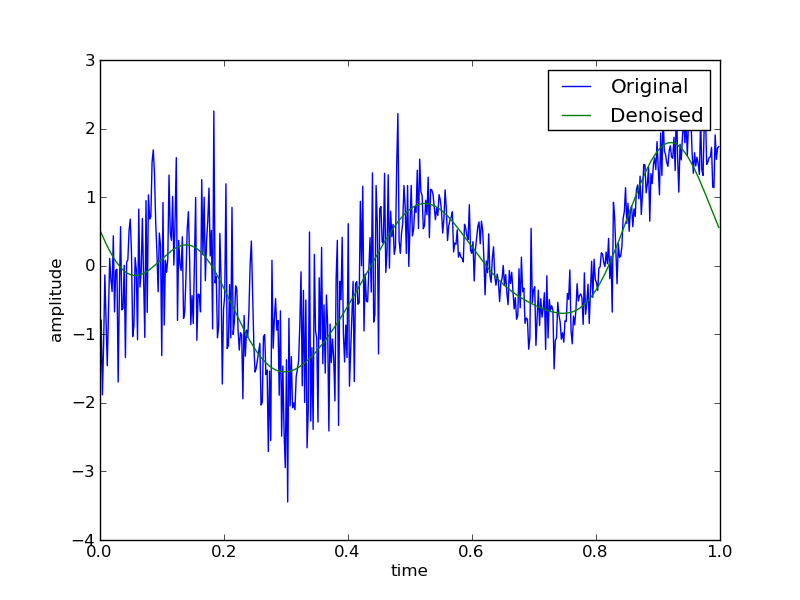
\includegraphics[width=\columnwidth]{denoised_signal_1d}
%  \caption{Signal compression and denoising using the Fourier basis.}
%  \vspace{-3mm}
%  \label{fig:denoise-fourier}
%\end{figure}
%\begin{figure}[htbp]
%  \centering
%  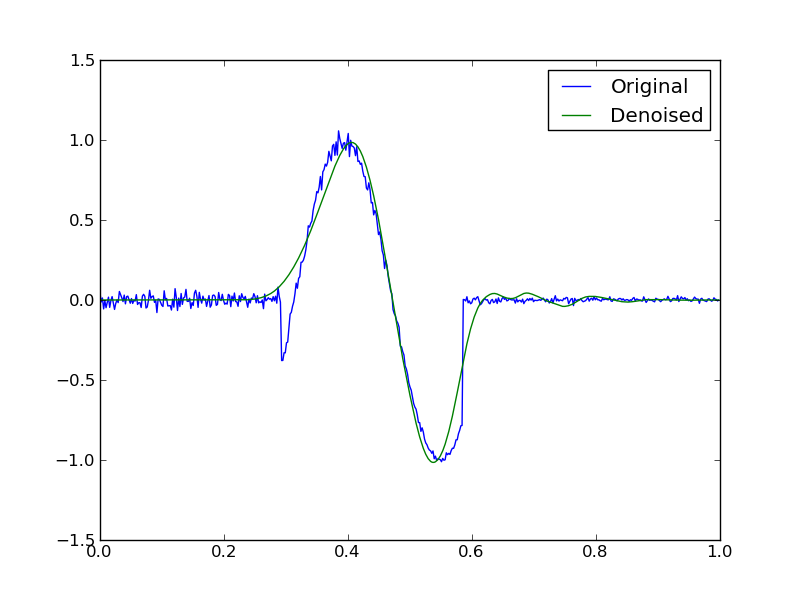
\includegraphics[width=\columnwidth]{local_wdenoised_1d}
%  \vspace{-3mm}
%  \caption{Signal compression and denoising using the Daubechies wavelet basis.}
%  \label{fig:denoise-wavelet}
%\end{figure}


%\begin{table*}[htbp]
%  \centering
%  \begin{tabular}[c]{|l||l|l|l|}
%    \hline
%    Basis&Support&Suitable signals&Unsuitable signals\\
%    \hline
%    Fourier&global&sine like&localized\\
%    wavelet&local&localized&sine like\\
%    \hline
%  \end{tabular}
%  \caption{Characteristics of Fourier and wavelet basis.}
%  \label{tab:fourier-wavelet}
%\end{table*}

%\section*{Acknowledgements}
%The author thanks Christian Sigg for his careful reading and helpful
%suggestions.

\bibliographystyle{IEEEtran}
\bibliography{literature}

\end{document}
